% !TEX program = xelatex
\documentclass[a4paper]{article}
\usepackage{amsmath}
\usepackage{amsthm}
\usepackage[left=1.8cm,right=1.8cm,top=2.2cm,bottom=2.0cm]{geometry}
\usepackage{ctex}
\usepackage{enumerate}
\usepackage{fancyhdr}
\usepackage{xpatch}
\usepackage{graphicx} 
\usepackage{float} 
\usepackage{subfigure} 
\usepackage{amsfonts}
\usepackage{mathtools}
\usepackage{framed}
\usepackage{multicol}
\usepackage{listings}
\usepackage{hyperref}
\usepackage{tikz}
\usetikzlibrary{automata,positioning}
\theoremstyle{definition}
\newtheorem*{solution*}{\textbf{Solution:}}
\newtheorem*{proof*}{\textbf{Proof:}}
\newtheorem{theorem}{Theorem}[subsection]
\newtheorem{definition}{Definition}[subsection]
\newtheorem{lemma}{Lemma}[subsection]
\makeatletter

\AtBeginDocument{\xpatchcmd{\@thm}{\thm@headpunct{.}}{\thm@headpunct{}}{}{}}
\makeatother

\pagestyle{fancy}
\renewcommand{\baselinestretch}{1.15}

\usepackage{paralist}
\let\itemize\compactitem
\let\enditemize\endcompactitem
\let\enumerate\compactenum
\let\endenumerate\endcompactenum
\let\description\compactdesc
\let\enddescription\endcompactdesc

% shorten footnote rule
\xpatchcmd\footnoterule
  {.4\columnwidth}
  {1in}
  {}{\fail}

\title{CS 131 Compilers: Discussion 8: Intermediate Representations: Basic Block and CFG \& Mid Term Preparation2}
\author{\textbf{杨易为}~~\textbf{季杨彪}~~\textbf{尤存翰} \\ \texttt{ \{yangyw,jiyb,youch\}@shanghaitech.edu.cn}}


\begin{document}
\maketitle
\section{Intermediate Representations}
An Intermediate Representation (IR) is an intermediate (neither source nor target) form of a program. There are various types of IRs:
\begin{enumerate}
  \item Section
  \begin{enumerate}
    \item \textbf{Abstract Syntax Trees} (AST): a simplified Parse Tree.\\
    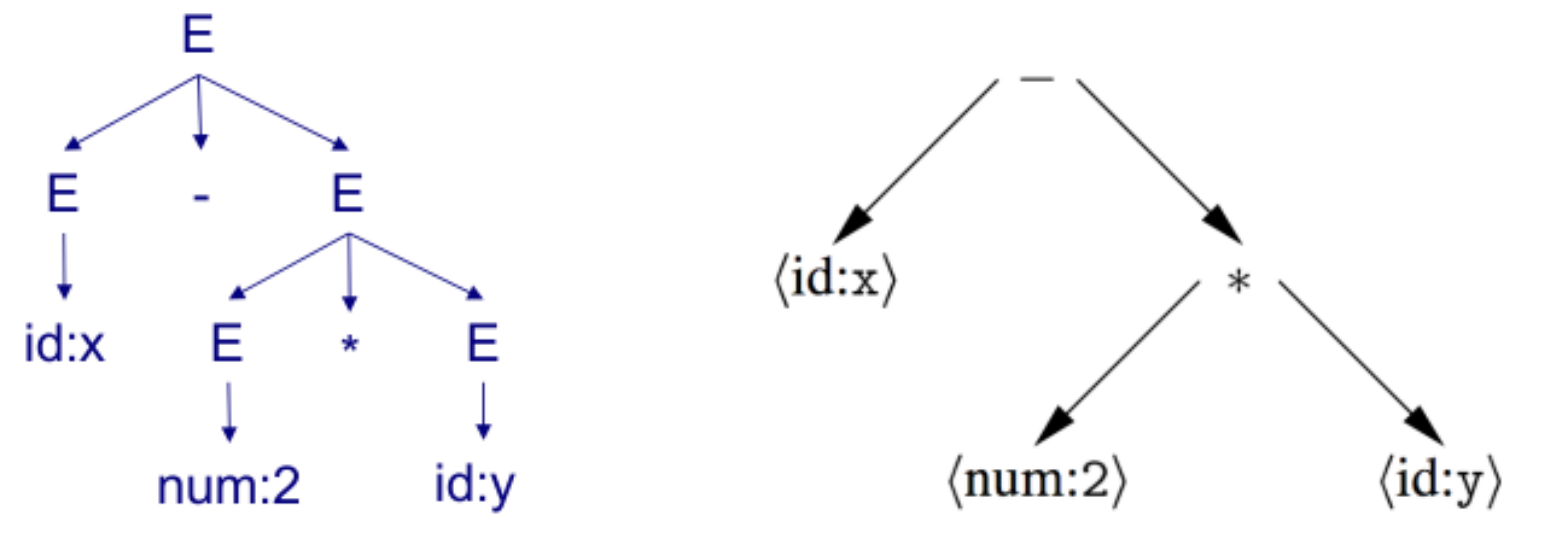
\includegraphics[width=10cm]{img/Snipaste_2021-04-19_07-08-30.png}
    \begin{itemize}
      \item + close to source compactdesc
      \item + suitable for source-source translation
      \item - Traversal \& Transformations are expensive
      \item - Pointer-intensive
      \item - Memory-allocation-intensive
    \end{itemize}

    \item \textbf{Directed Acyclic Graphs} (DAG): DAG is an optimized AST, with identical nodes \textit{shared}.\\
    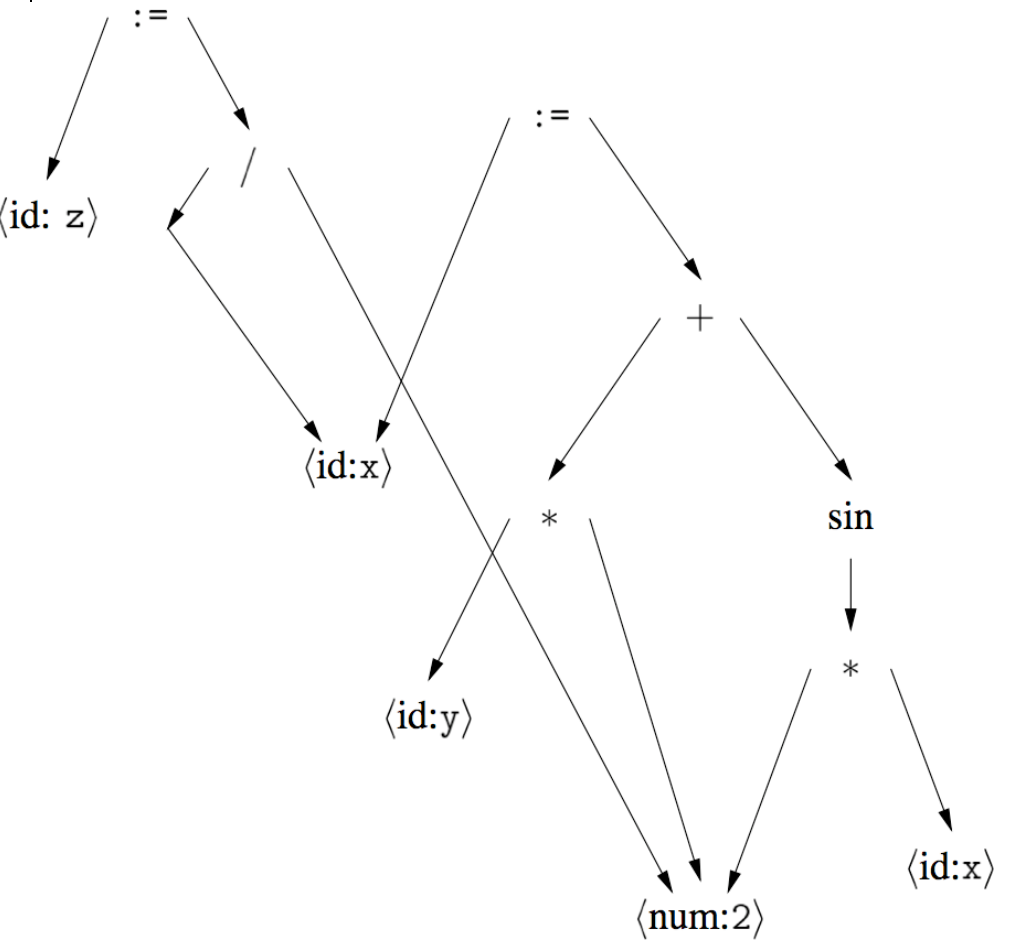
\includegraphics[width=10cm]{img/Snipaste_2021-04-19_07-11-03.png}
    \begin{itemize}
      \item + Explicit sharing
      \item + Exposes redundancy, more efficient, useful for dynamic pipelining analysis
      \item - Difficult to transform
      \item - Analysis usage Practical usage
    \end{itemize}
    \item \textbf{Control Flow Graphs} (CFG): CFG is a flow chart of program execution. Is a conservative approximation of the Control Flow, because only one branch will be actually executed.\\
    A Basic Block is a consecutive sequence of Statements $S_{1}, \ldots, S_{n}$, where flow must enter this block only at $S_{1}$, AND if $S_{1}$ is executed, then $S_{2}, \ldots, S_{n}$ are executed strictly in that order, unless one Statement causes halting.

    \begin{itemize}
      \item The Leader is the first Statement of a Basic Block
      \item A Maximal Basic Block is a maximal-length Basic Block
    \end{itemize}
    Nodes of a CFG are Maximal Basic Blocks, and Edges of a CFG represent control flows
    \begin{itemize}
      \item $\exists$ edge $b_{1} \rightarrow b_{2}$ iff control may transfer from the last Statement of $b_{1}$ to the first Statement of $b_{2}$
    \end{itemize}
    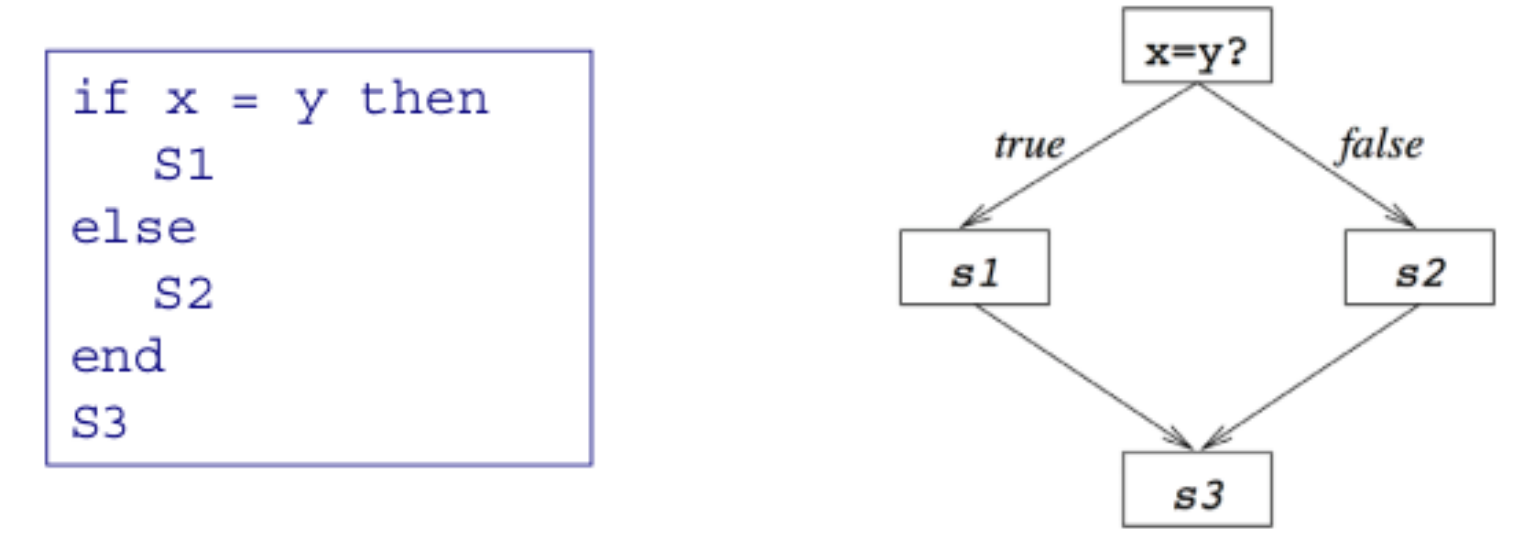
\includegraphics[width=10cm]{img/Snipaste_2021-04-19_07-14-56.png}
    \begin{itemize}
      \item + Most widely used form. Can cast \href{https://chhzh123.github.io/blogs/2020-03-24-spa-nju/}{static analysis} on it.
    \end{itemize}
    \item \textbf{Single Static Assignment} (SSA): SSA means every variable will only be assigned value ONCE (therefore single). Useful for various kinds of optimizations.\\
    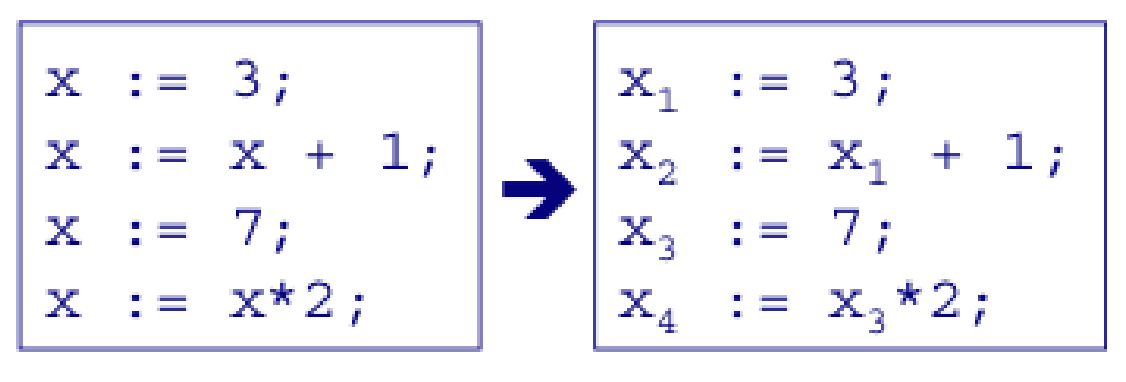
\includegraphics[width=10cm]{img/Snipaste_2021-04-19_17-49-29.png}
    A $\phi$ -function generates an extra assignment to "choose" from Branches or Loops. If Basic Block $B$ has Predecessors $P_{1}, \ldots, P_{n}$, then $X=\phi\left(v_{1}, \ldots, v_{n}\right)$ assigns $X=v_{j}$ if control enters $B$ from $P_{j}$.\\
    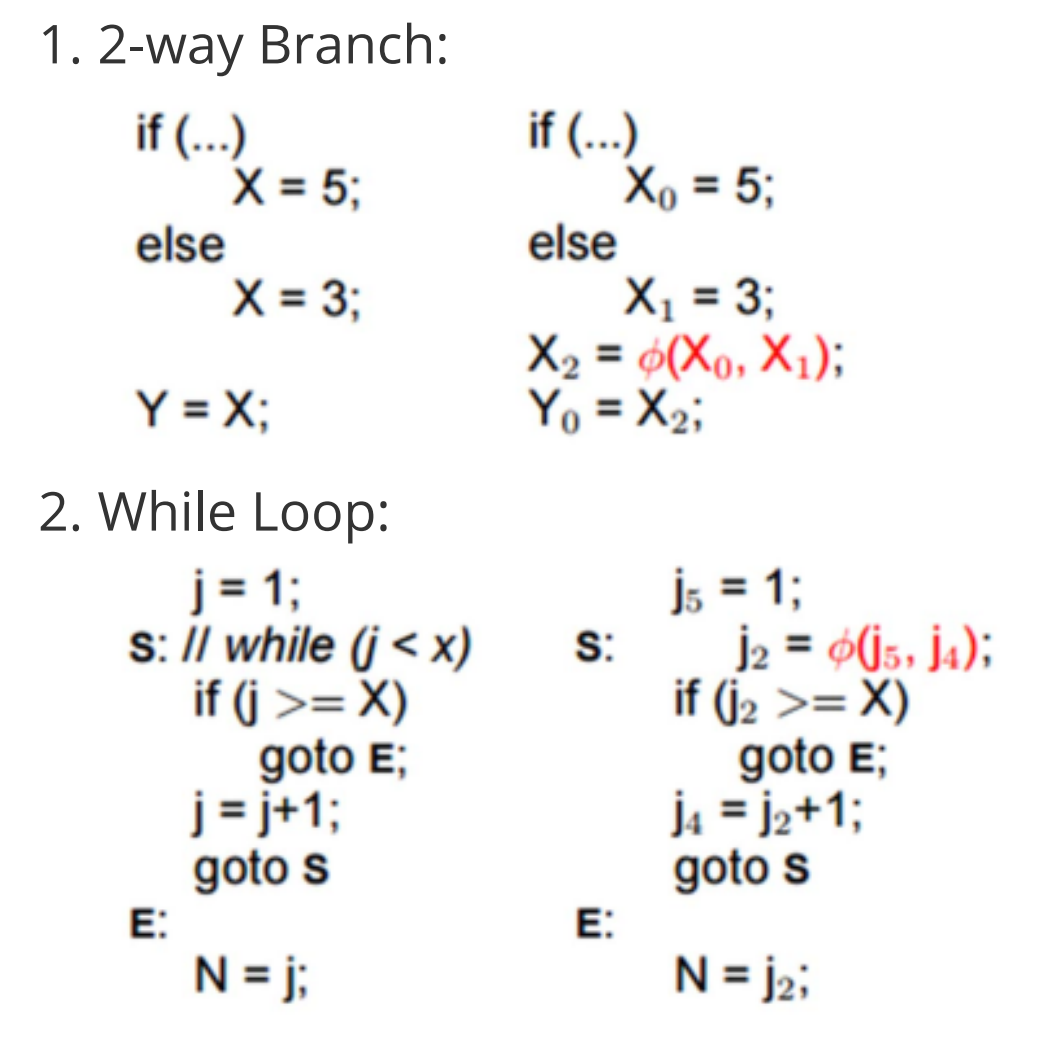
\includegraphics[width=10cm]{img/Snipaste_2021-04-19_17-50-16.png}
    \begin{enumerate}
      \item $\phi$ is not an executable operation
      \item Number of $\phi$ arguments $=$ Number of incoming edges
      \item Where to place a $\phi ?$ If Basic Block $B$ contains an assignment to variable $X$, then a $\phi$ MUST be inserted before each Basic Block $Z$ that:\\
      1. $\exists$ non-empty path $B \rightarrow^{+} Z$\\
      2. $\exists$ path from ENTRY to $Z$ which does not go through $B$\\
      3. $Z$ is the FIRST node that satisfies $\mathrm{i}$. and ii.
    \end{enumerate}
  \end{enumerate}
\end{enumerate}
\section{Mid Term Preparation2 }
\subsection {LR(1) parsing}
\textbf{Build $L R(1)$ Automaton:}
An $L R(1)$ Item $(i, a)$ is an extension of $L R(0)$ Item, where the next allowed Token $a$ is considered.
$i$ is a $L R(0)$ item, $a$ is an input Terminal, allowing Reduction using $i$ when input is $a$
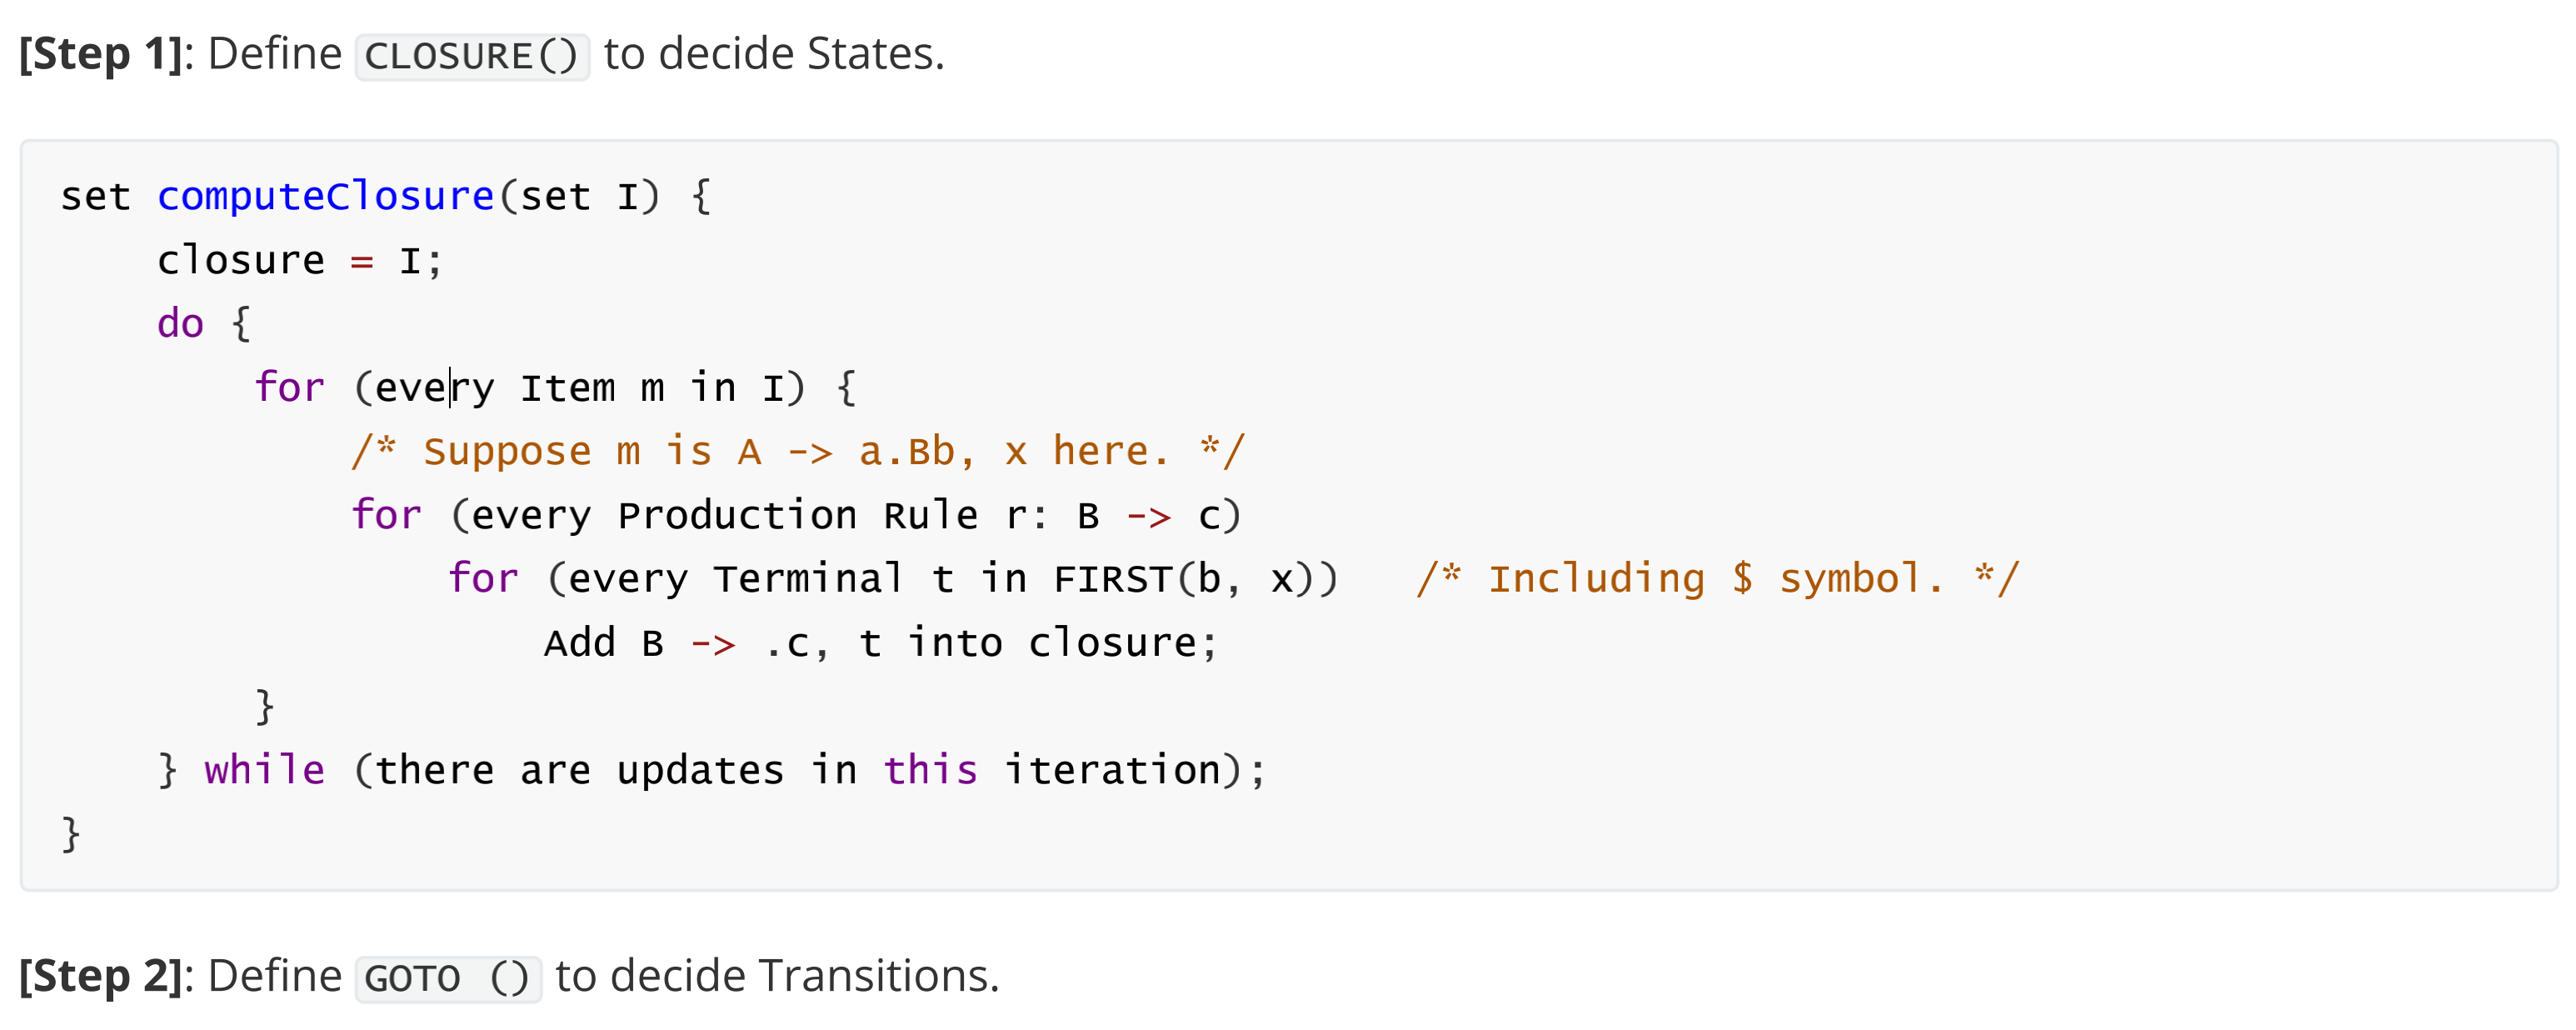
\includegraphics[width=15cm]{img/Snipaste_2021-04-19_17-56-00.png}\\
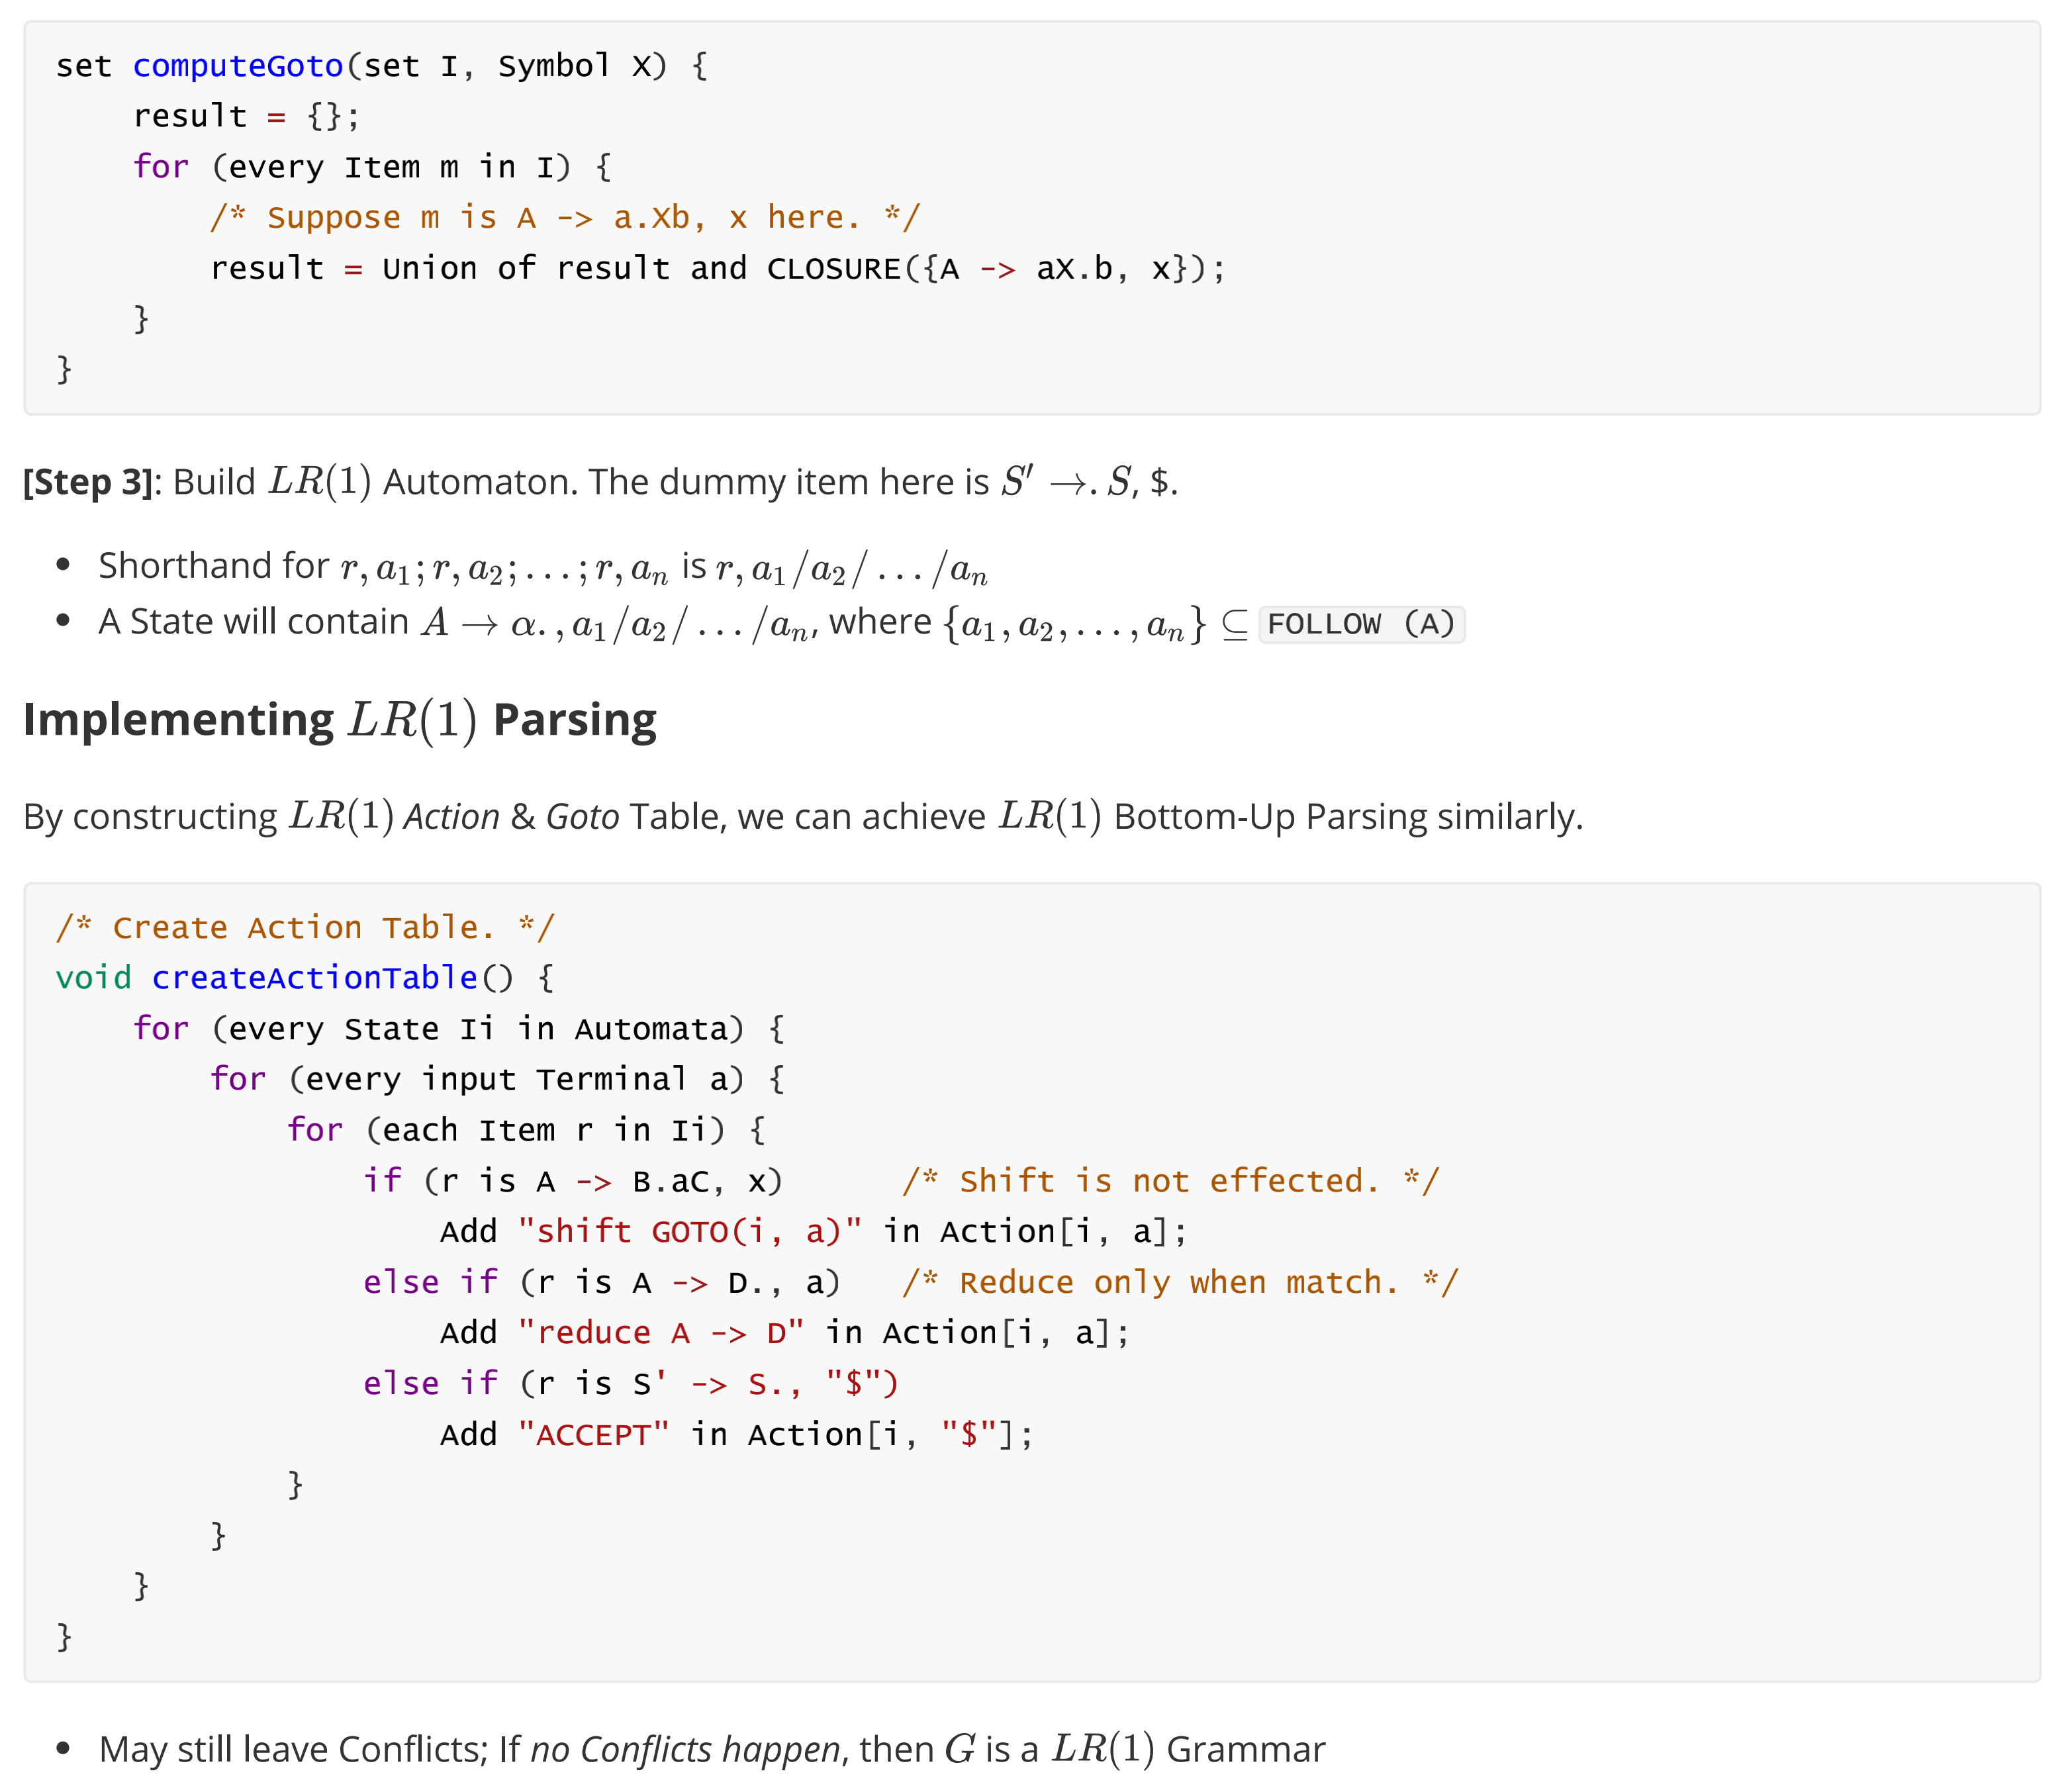
\includegraphics[width=15cm]{img/Snipaste_2021-04-19_17-56-46.png}
\subsection {LALR(1) parsing}
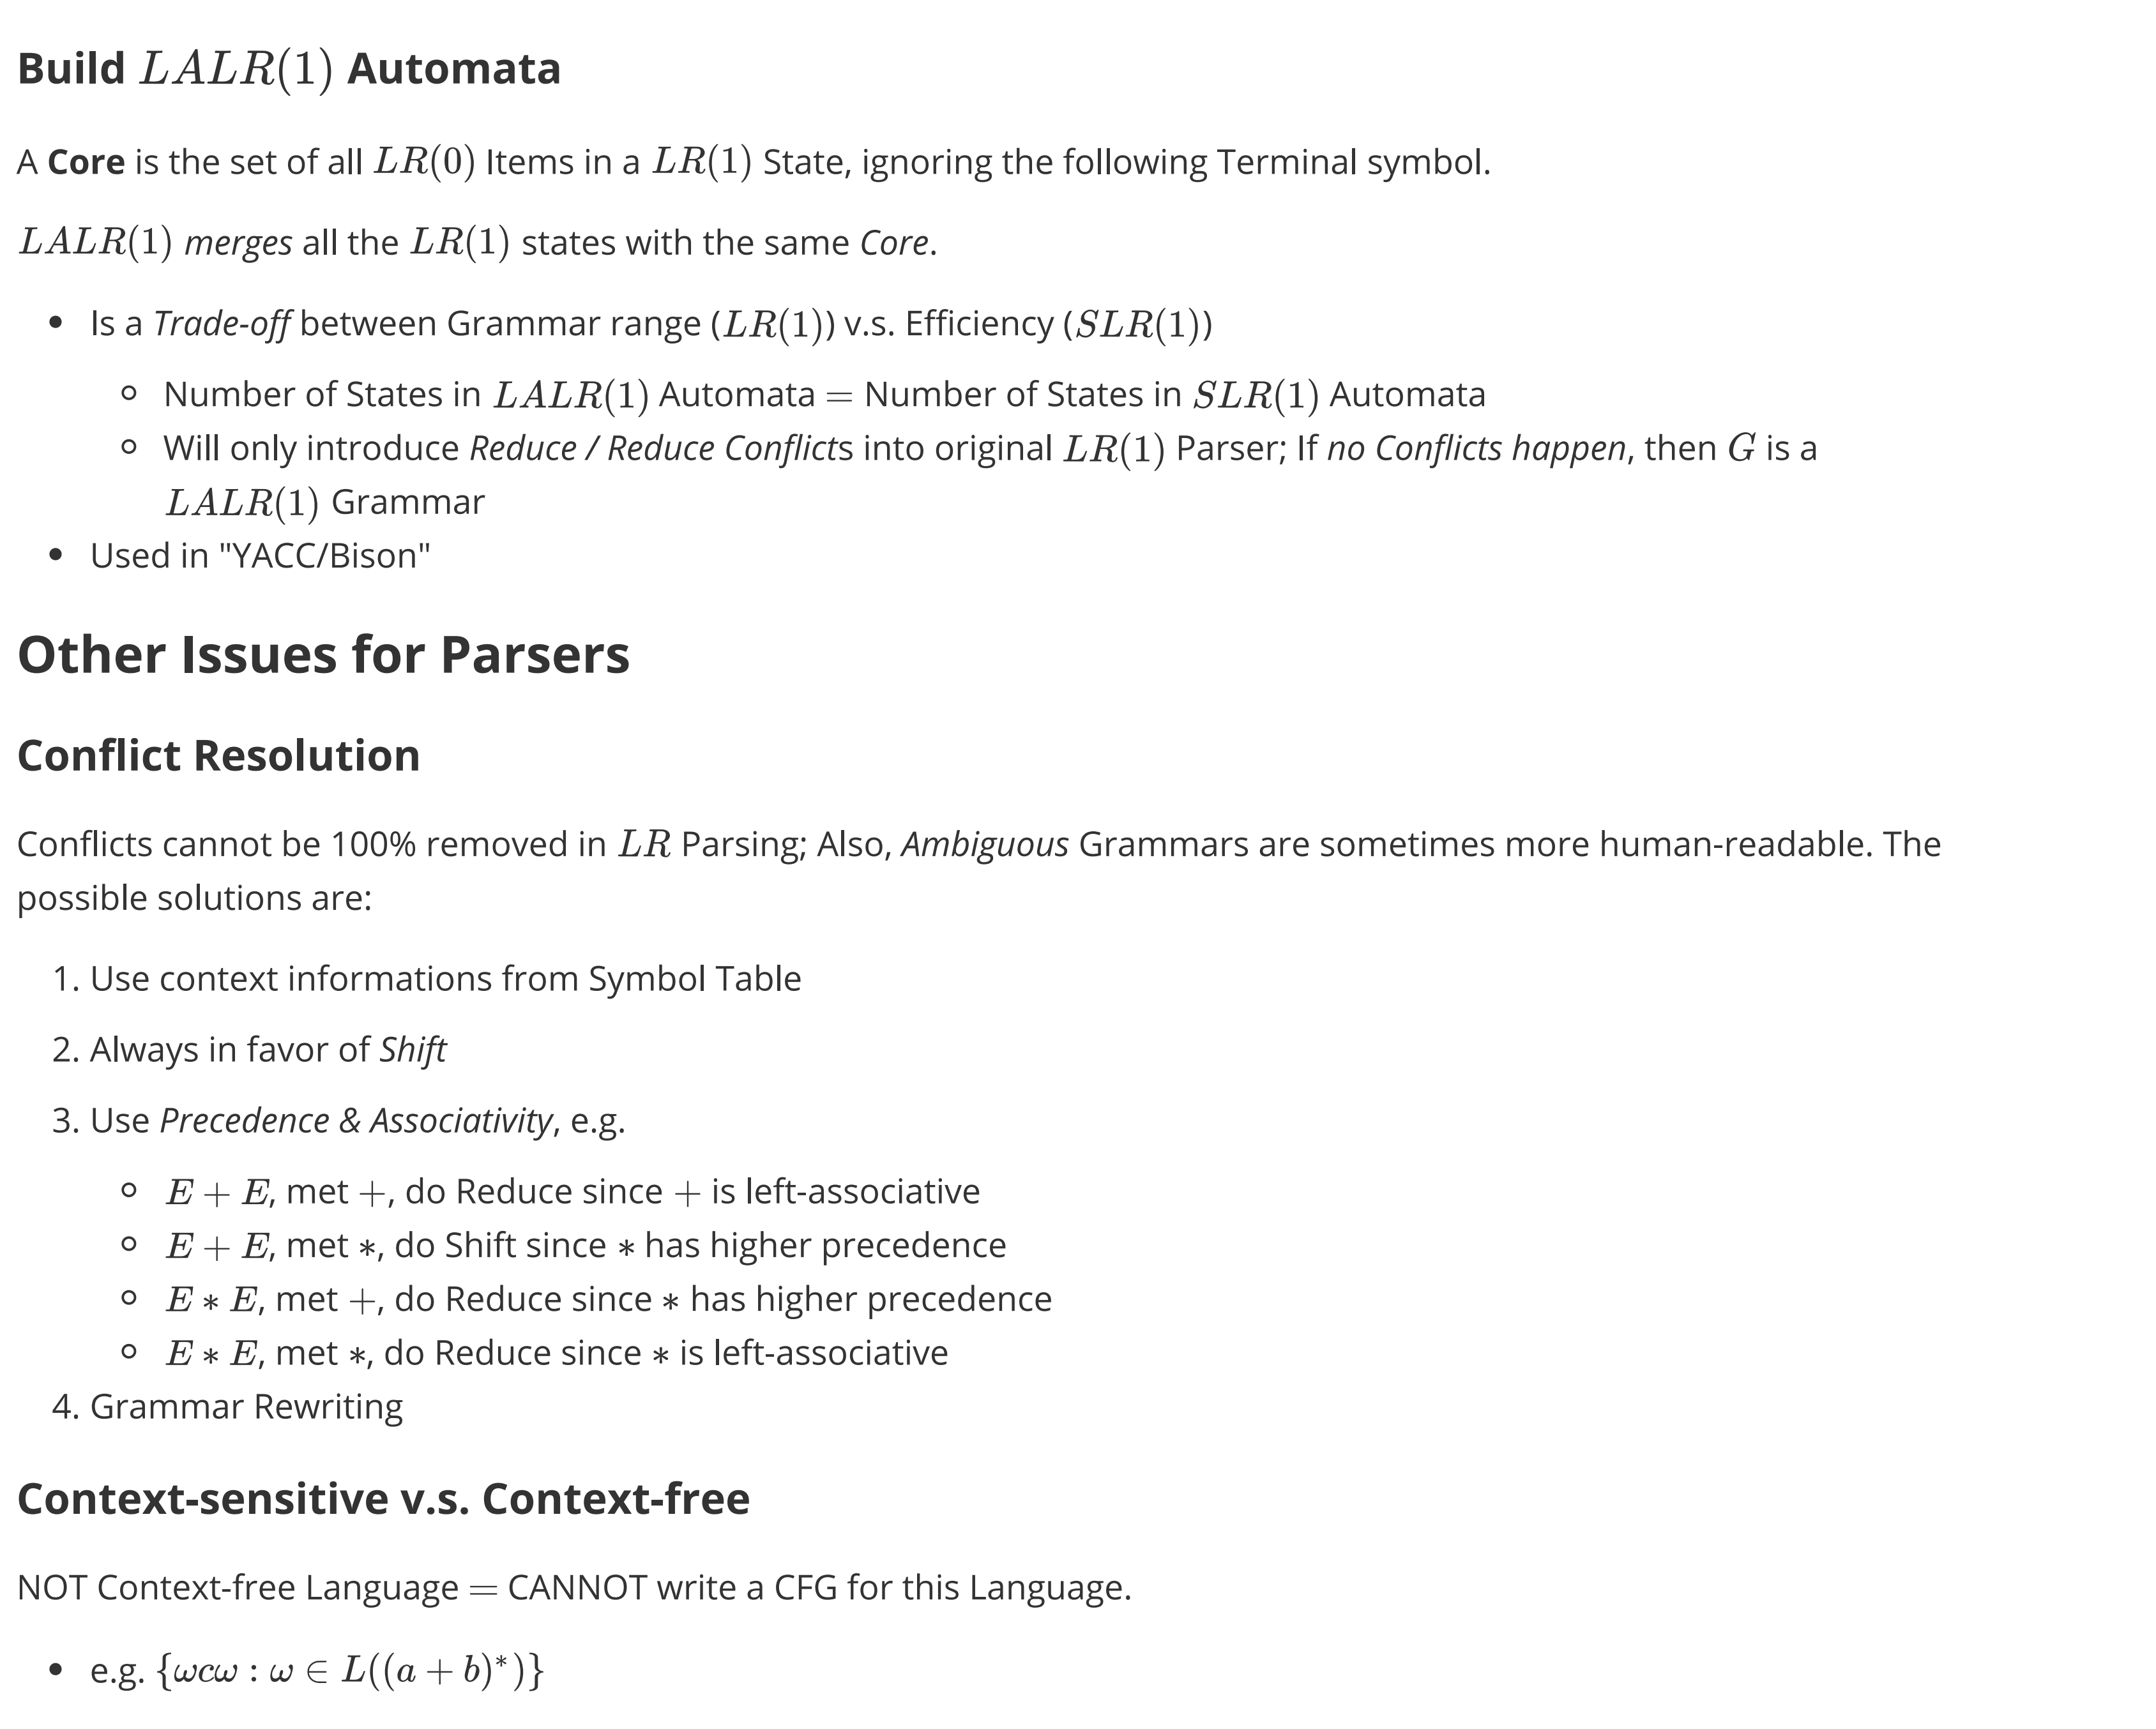
\includegraphics[width=15cm]{img/Snipaste_2021-04-19_17-57-34.png}
\end{document}
